%BAB_2 LAPORAN KP
\chapter{LANDASAN TEORI}

\section{Gambaran Umum Robot Lengan}

Robot adalah adalah sebuah alat yang terdiri dari gabungan mekanik dan elektronik yang dapat melakukan tugas fisik, baik menggunakan pengawasan dan kendali manusia maupun secara otomatis. Robot dapat melakukan suatu tugas secara berulang tanpa merasa lelah sehingga robot banyak digunakan dalam dunia industri khususnya pada bidang produksi. Salah satu jenis robot yang sering dalam bidang produksi adalah sistem lengan robot.

Robot lengan adalah robot yang memiliki bentuk fisik seperti halnya lengan pada manusia dan memiliki derajat kebebasan (degre of freedom) tertentu bergantung pada jumlah sendi yang digunakan. Dengan begitu robot lengan terdiri dari beberapa jenis. Robot lengan pada bidang industri biasa digunakan sebagai actuator untuk mengambil dan meletakkan suatu objek secara terus menerus.
	

Pada umumnya struktur robot lengan terdiri dari beberapa bagian.  Bagian utama adalah struktur mekanik (manipulator) yang merupakan susunan kerangka yang tidak dapat digerakkan (rigid) dan lengan (link) yang satu sama lain terhubung oleh sendi (joint). Dengan adanya joint yang menghubungkan dua link menjadi satu kesatuan sehingga joint membentuk satu derajat kebebasan. Jika diibaratkan dengan tubuh manusia, link adalah tulang sedangkan joint adalah sendi-sendinya. Joint memiliki dua pergerakan, yaitu pergerakan revolute joint (gerak berputar) dan prismatic joint (gerak bergeser) seperti yang ditunjukkan oleh Gambar 2.1

	\begin{figure}[H]
	\centering
	\includegraphics[width=5cm]{gambar/joint.png}
	\caption{Jenis-Jenis \emph Joint}
\end{figure}

Pada ujung pangkal lengan, robot lengan umumnya menggunakan gripper yang dapat dipakai untuk memindahkan suatu objek. Robot lengan dalam menjalankan tugasnya dikontrol menggunakan sensor serta aktuator yang telah dirancang untuk melakukan tugas sesuai dari yang diperintahkan. Perpaduan antara sensor dan aktuator ini yang menyebabkan robot lengan dapat bekerja secara optimal dan presisi.

\subsection{\emph{Degress of Freedom }}
Degress of freedom (DOF) merupakan sebuah konfigurasi yang dapat meminimalkan spesifikasi dengan menggunakan n parameter yang dapat menyatakan posisi suatu system pada setiap saat. Biasanya, robot lengan mempunyai paling sedikit enam independen derajat kebebasan: tiga derajat kebebasan untuk translasi dan tiga derajat kebebasan untuk rotasi. Umumnya untuk robot lengan paling tidak memiliki tiga derajat kebebasan untuk dapat memiliki workspace yang cukup. Workspace dari sebuah robot lengan merupakan total volume yang dapat dijangkau oleh end effector dari pergerakan semua jointnya dari titik minimum hingga maksimum. 

\subsection{Konfigurasi Robot Lengan}
Pada dasarnya, berbagai jenis dari robot lengan dapat dibedakan dari konfigurasinya. konfigurasi robot lengan merupakan perpaduan antara pergerakan joint yang dimiliki oleh robot lengan. konfigurasi ini memiliki tipe yang berbeda-beda sehingga \emph workspace yang dimiliki pada tiap robot lengan pasti berbeda.

\subsubsection{A. Konfigurasi Articulated (Revolute - Revolute - Revolute)} 
Articulated manipulator ini pada dasarnya mempunyai jenis revolute joint pada ketiga joint robot lengan (\emph {wrist, shoulder, elbow}). Dengan konfigurasi ini, robot lengan dengan konfigurasi Articulated dapat memiliki variasi DOF yang banyak. DOF yang daoat dihasilkan dengan robot lengan dengan konfigurasi seperti ini adalah tiga DOF hingga sampai dengan enam DOF tergantung dari kebutuhan dan fungsi yang akan dilakukan oleh robot lengan. Konfigurasi dari joint revolute ini menjadikan robot lengan jenis ini mempunyai kebebasan yang besar dari pergerakannya dalam ruang yang kecil sehingga menjadikan jenis konfigurasi articulated manipulator ini banyak dipakai dan memiki desain yang populer. Konfigurasi Articulated ini dapat dianalisakan seperti yang ada pada Gambar 2. 2.
	\begin{figure}[H]
	\centering
	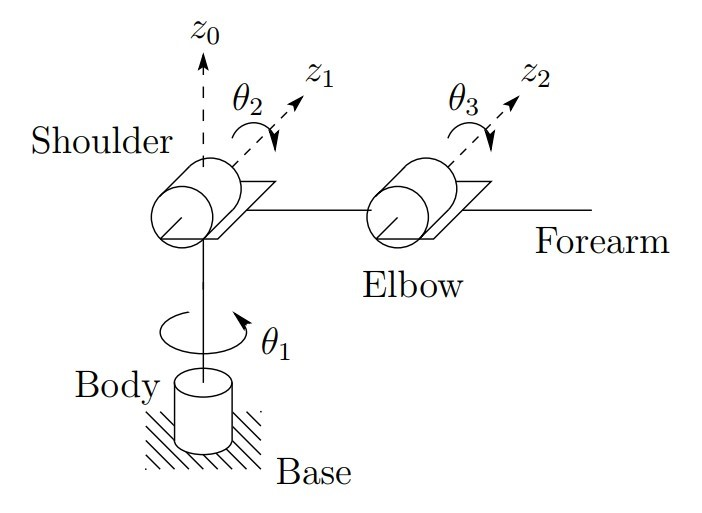
\includegraphics[width=5cm]{gambar/articulated.jpg}
	\caption{Struktur dari Konfigurasi \emph Articulated}
\end{figure}
\subsubsection{B. Konfigurasi Spherical (Revolute – Revolute – Prismatic)   )} 

Konfigurasi spherical merupakan konfigurasi yang mempunyai dua buah joint revolute dan satu buah joint prismatic. Joint prismatic berada ini joint ketiga atau pada bagian elbow. Sementara dua joint lainnya berada di shoulder dan waist. Sruktur dari konfigurasi Spherical seperti pada Gambar 2.3
	\begin{figure}[H]
	\centering
	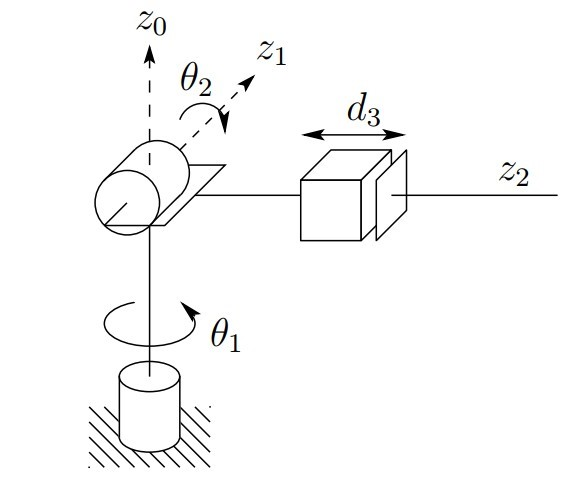
\includegraphics[width=5cm]{gambar/spherical.jpg}
	\caption{Struktur dari\emph Sperical}
\end{figure}


\subsubsection{C. Konfigurasi SCARA (Revolute – Revolute – Prismatic) } 

Konfigurasi Selective Compliant Articulated Robot for Assembly (SCARA) merupakan konfigurasi yang mempunyai dua buah joint revolute dan satu buah joint prismatic sama seperti konfigurasi Spherical. Meskipun SCARA memiliki struktur joint revolute – revolute – prismatic (RRP) sama seperti konfigurasi yang dimiliki spherical, struktur ini sedikit berbeda dengan konfigurasi spherical dari tampilannya maupun dari jarak workspace nya. Tidak seperti konfigurasi spherical, dimana z0 tegak lurus terhadap 1, dan z1 tegak lurus dengan z2, konfigurasi SCARA memiliki struktur z0, z1, dan z2 yang paralel. Struktur dari konfigurasi SCARA seperti yang ditunjukkan Gambar 2.4
	\begin{figure}[H]
	\centering
	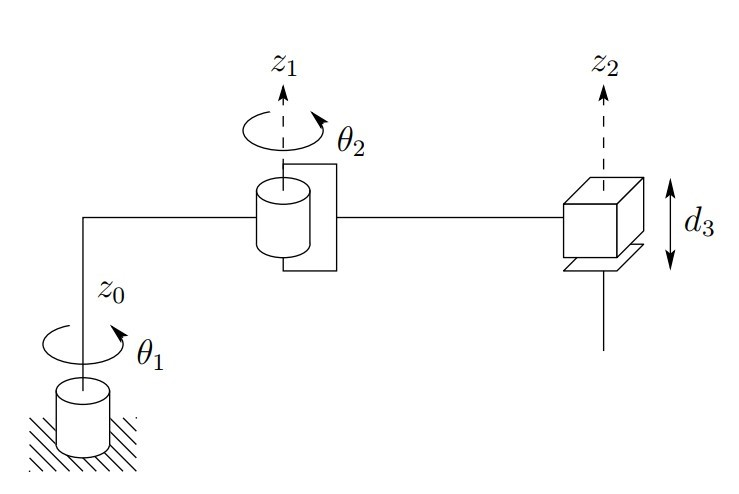
\includegraphics[width=5cm]{gambar/scara.jpg}
	\caption{Struktur dari Konfigurasi \emph SCARA}
\end{figure}

\subsubsection{D. Konfigurasi Cylindrical (Revolute – Prismatic – Prismatic) } 

Konfigurasi Cylindrical merupakan konfigurasi yang mempunyai satu buah joint revolute dan dua buah joint prismatic. Joint revolute menghasilkan pergerakan rotasi di base/ waist, sementara joint prismatic berada di bagian shoulder dan elbow. Struktur dari konfigurasi Cylindrical seperti yang ditunjukkan oleh Gambar 2.5
	\begin{figure}[H]
	\centering
	\includegraphics[width=5cm]{gambar/cylindrical.jpg}
	\caption{Struktur dari Konfigurasi \emph Cylindrical}
\end{figure}
\subsubsection{E. Konfigurasi Cartesian (Prismatic – Prismatic – Prismatic)  } 

Konfigurasi cartesian mempunyai tiga buah joint prismatic. Variabel joint dari konfigurasi prismatic adalah koordinat cartesian dari end-effector dengan memperhatikan letak base dari robot lengan. Seperti yang diperkirakan kinematika dari jenis konfigurasi ini adalah yang paling sederhana dari semua konfigurasi robot lengan. Konfigurasi cartesian sangat berguna untuk penyusunan suatu barang di bidang datar seperti mesin laser, kargo atau memindahkan barang. Struktur dari konfigurasi Cartesian ditunjukkan pada Gambar 2.6

	\begin{figure}[H]
	\centering
	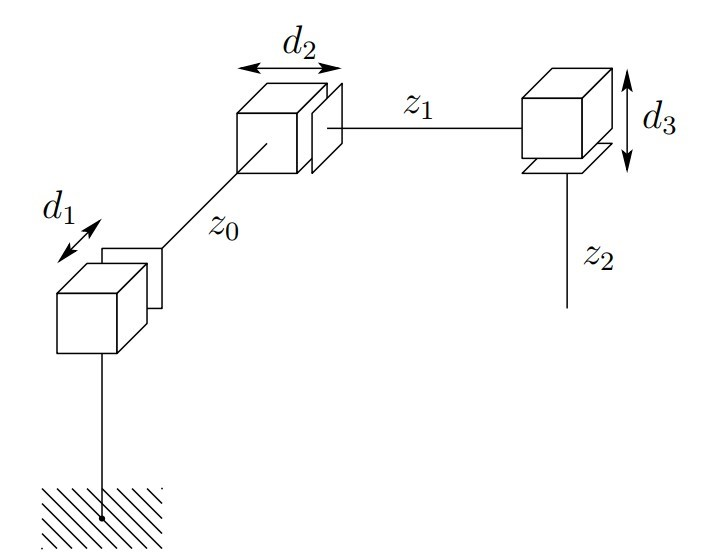
\includegraphics[width=5cm]{gambar/cartesian.jpg}
	\caption{Struktur dari Konfigurasi \emph Cartesian}
\end{figure}

\subsection{ Wrist dan End-effector }

Wirst atau pergelangan tangan merupakan joint diantara lengan dan end-effector. Joint wrist ini pada umumnya terdapat joint revolute . Hal ini umum digunakan pada desain manipulator lengan dengan konfigurasi spherical. Konfigurasi spherical mempunyai joint revolute yang saling berpotongan diantara ketiganya, maksudnya setiap joint berputar sesuai koordinat x, y dan z. rotasi atau perputaran dengan axis sumbu x adalah roll, perputaran dengan axis sumbu y adalah pitch dan perputaran dengan axis sumbu z adalah yaw. Joint spherical wrist ini dijelaskan pada Gambar 2. 7.
	\begin{figure}[H]
	\centering
	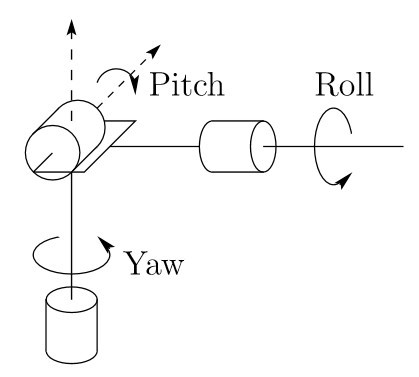
\includegraphics[width=5cm]{gambar/wirst.jpg}
	\caption{Struktur dari Joint Spehrical Wrirst}
\end{figure}


End-effector merupakan perangkat atau alat yang terhubung dengan ujung lengan robot. End-effector adalah bagian robot yang berhubungan langsung dengan objek. Struktur, pergerakan, material dari end-effector bergantung pada tugas yang akan dilakukan robot tersebut. Stuktur dan bentuk dari end-effector seperti yang ditunjukkan pada Gambar 2.8


\section{Kinematika}
Kinematika merupakan pembelajaran pergerakan tubuh tanpa memperhitungkan gaya, torsi maupun momen tertentu yang menyebabkan pergerakan. Terdapat berbagai jenis pergerakan dari kinematika tergantung dari tujuan dari setiap robot. Kinematika yang akan dijelaskan disini adalah kinematika yang khusus mempelajari dan menganalisa pergerakan lengan robot lengan.  

Pada kinematika robot, terdapat dua buah pembahasan kinematika. Pembahasan pertama adalah kinematika maju merupakan proses menghitung orientasi dan posisi dari end-effector berdasarkan sudut-sudut dari joint.  Sedangkan kinematika balik sebaliknya dari kinematika maju, diberikan posisi end-effector, dimana yang akan dicari adalah besaran sudut yang harus diubah untuk tiap joint dalam mencapai posisi end-effector tersebut.Diagram blok sederhana dari pemodelan kinematika ditunjukkan pada Gambar 2.9
	\begin{figure}[H]
	\centering
	\includegraphics[width=5cm]{gambar/kinematika_diagram.png}
	\caption{Blok Diagram Kinematika Balik}
\end{figure}

\subsection{Kinematika Maju}
Kinematika maju atau biasa disebut forward kinematics merupakan kinematik untuk mendapatkan hasil akhir berupa koordinat posisi (x, y, z) dengan diketahuinya variabel sudut pada setiap joint dari lengan robot.  Variabel sudut tersebut kemudian dilakukan perhitungan satu sama lain hingga pada akhirnya akan mendapatkan koordinat x, koordinat y, dan koordinat z. Proses dari kinematika maju dapat ditunjukkan pada Gambar 2.10
	\begin{figure}[H]
	\centering
	
\includegraphics[width=5cm]{gambar/Kinematika_maju.png}
	\caption{Kinematika Maju}
\end{figure}


\subsection{Kinematika Balik}
Kinematika Balik Kinematika balik (inverse kinematics) digunakan untuk mencari variabel sudut (joint) robot dalam menentukan posisi dan orientasi dari end-effector. Dalam menentukan koordinat end-effector, kinematika balik mengacu pada penggunaan persamaan kinematika robot untuk menentukan parameter bersama yang memberikan posisi yang diinginkan pada posisi akhir atau end-effector. Kinematika balik mengubah rencana gerak menjadi nilai yang harus diberikan bagi aktuator atau penggerak dalam pergerakan robot.  Dalam pergerakannya , robot dimodelkan dalam bentuk persamaan kinematika. Persamaan ini menentukan konfigurasi robot dalam hal parameter untuk setiap aktuator. Kinematika maju menggunakan parameter untuk menghitung konfigurasi robot, dan kinematika balik membalikkan perhitungan ini untuk menentukan parameter bersama dalam mencapai konfigurasi yang diinginkan. 

Secara garis besar metode kinematika balik akan mencari nilai-nilai parameter yang harus diberikan kepada setiap aktuator untuk mencapai tujuan akhir. Untuk mendapatkan nilai-nilai parameter tersebut, robot harus mengetahui terlebih dahulu manipulator yang dimilikinya, baik ukuran maupun jumlah aktuator serta derajat kebebasan yang ada. Kemudian, robot harus ditanamkan rumus-rumus yang didapat dari berbagai model perhitungan, baik dari segi analisa grafik langsung maupun menggunakan metode-metode dari berbagai penelitian. Proses dari kinematika balik seperti yang ditunjukkan pada Gambar 3.1

	\begin{figure}[H]
	\centering
	\includegraphics[width=5cm]{gambar/kinematika_balik.png}
	\caption{Kinematika Balik}
\end{figure}

\section{Motor DC}
Motor DC adalah motor listrik yang memerlukan suplai tegangan arus searah pada kumparan medan untuk diubah menjadi energi gerak mekanik. Motor DC mempunyai dua bagian utama, yaitu stator dan rotor. Stator merupakan bagian yang tidak berputar dan rotor merupakan bagian yang berputar dan merupakan kumparan jangkar. Motor DC menghasilkan jumlah putaran dalam setiap satuan waktu yang biasanya dihitung setiap satuan menit (rotations per minute) dan dapat diatur arah putaranya searah jarum jam (clock wise) atau berkebalikan dengan arah jarum jam (counter clock wise) bergantung dengan kutub atau polaritas dari catu daya yang diberikan pada motor DC. Bentuk dari motor DC dapat ditunjukkan pada Gambar 4.1
	\begin{figure}[H]
	\centering
	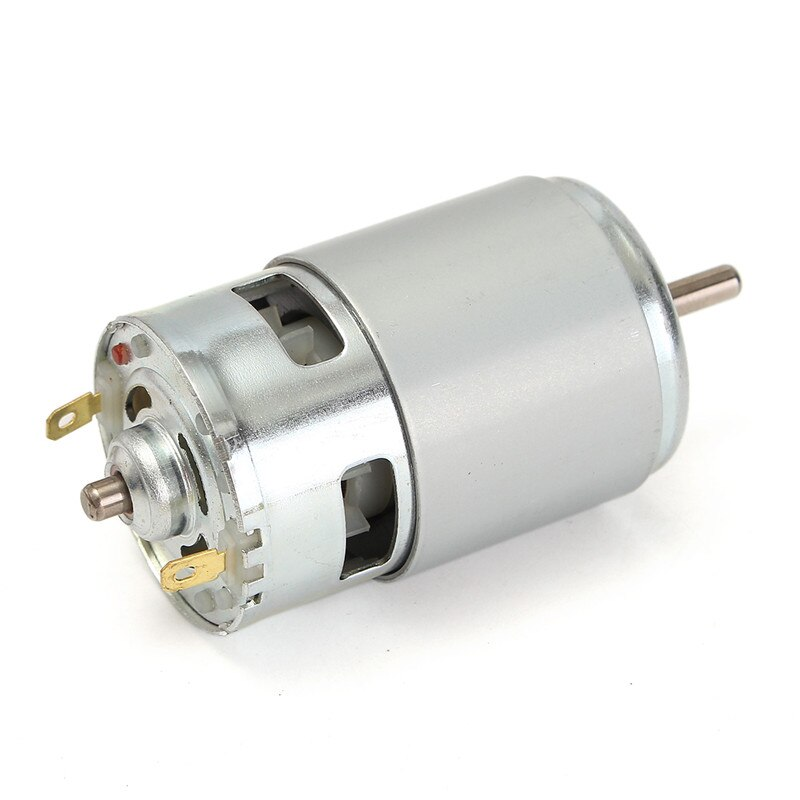
\includegraphics[width=5cm]{gambar/motorDC.jpeg}
	\caption{Jenis-Jenis \emph Joint}
\end{figure}

Motor DC dapat bergerak karena adanya elektromagnet. Saat kumparan diberi arus listrik, permukaan kumparan yang bersifat utara akan bergerak menghadap ke magnet yang berkutub selatan dan kumparan yang bersifat selatan akan bergerak menghadap ke utara magnet. Saat ini, kerena kedua kutub saling menyebabkan pergerakan kumparan berhenti. Untuk menggerakannya lagi, tepat pada saat kutub kumparan berhadapan dengan kutub magnet, arah arus pada kumparan dibalik. Dengan demikian, kutub utara kumparan akan berubah menjadi kutub selatan dan kutub selatannya akan berubah menjadi kutub utara.  

Pada saat perubahan kutub tersebut terjadi, kutub selatan kumparan akan berhadapan dengan kutub selatan magnet dan kutub utara kumparan akan berhadapan dengan kutub utara magnet. Karena kutubnya sama, maka akan terjadi tolak menolak sehingga kumparan bergerak memutar hingga utara kumparan berhadapan dengan selatan magnet dan selatan kumparan berhadapan dengan utara magnet. Siklus ini akan berulang-ulang hingga arus listrik pada kumparan diputuskan. Prinsip kerja motor DC dijelaskan pada Gambar 2.11.  
	\begin{figure}[H]
	\centering
	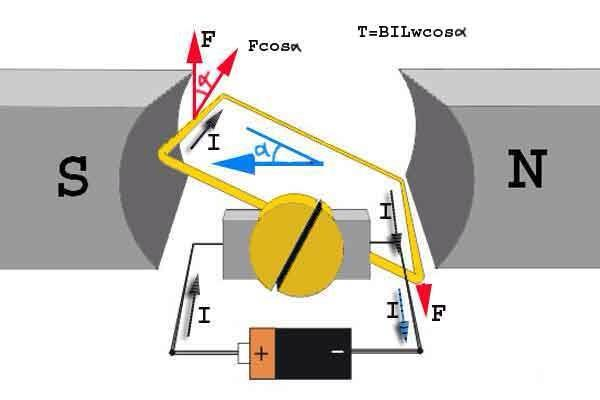
\includegraphics[width=5cm]{gambar/prinsipDC.jpg}
	\caption{Prinsip Kerja Motor DC}
\end{figure}


\section{Regulator}
Dalam suatu rangkaian elektronika dibutuhkan suatu sumber stabil dan sesuai dengan nilai yang dibutuhkan oleh komponen. Untuk memenuhi kebutuhan tersebut digunakanlah sebuah rangkaian regulator. Rangkaian regulator berfungsi untuk mengatur atau menghasilkan nilai tegangan pada nilai tertentu dari suatu tegangan masukan. Regulator dapat mempertahankan nilai tegangan yang keluar tanpa dipengaruhi besar arus yang dikeluarkannya. Regulator tegangan mempunyai banyak jenisnya, salah satunya adalah regulator switching.

Regulator switching mengatur besarnya nilai tegangan keluaran dengan mensaklar (ON/OFF) tegangan masukan dengan frekuensi berbeda – beda. Kelebihan dari regulator switching adalah mempunyai disipasi daya yang terjadi lebih kecil dibandingkan dengan regulator linear. Sedangkan kekurangan yaitu tegangan keluaranya akan berbentuk gelombang akibat adanya proses switching. Oleh karena itu, regulator jenis ini umumnya membutuhkan induktor, kapasitor , dan dioda untuk memperhalus tegangan keluaran. Regulator switching ada dua jenis yaitu regulator Buck dan regulator Boost. Regulator Buck untuk menghasilkan nilai tegangan keluaran yang lebih kecil dari tegangan masukannya. Sedangkan Regulator Boost untuk menghasilkan nilai tegangan yang lebih besar dari tegangan masukannya. Salah satu jenis dari regulator Buck adalah LM2596 . Bentuk fisik dari regulator Buck seperti yang ditunjukkan pada Gambar 3.2

	\begin{figure}[H]
	\centering
	\includegraphics[width=5cm]{gambar/lm2596.jpg}
	\caption{Jenis-Jenis \emph Joint}
\end{figure}

\section{Arduino}
Arduino  merupakan papan pengembangan dari mikrokontroler yang menggunakan basis Arduino serta menggunakan microchip At 2560. Arduino  memiliki pin input dan output dengan jumlah yang cukup banyak, yaitu sejumlah 54 buah pin input dan output yang 15 diantaranya merupakan pin pulse with modulation (PWM), 16 diantaranya merupakan pin analog input, dan terdapat empat pin yang digunakan sebagai UART (serial port hardware). Arduino ini sudah dilengkapi dengan oscillator sebesar 16Mhz, sebuah port usb, power jack DC, ICSP header serta tombol reset [17]. Gambar 2.13 Merupakan bentuk fisik Arduino .

Arduino merupakan papan pengembangan dari mikrokontroler yang menggunakan basis Arduino serta menggunakan microchip At 2560. Arduino memiliki beberapa jenis, salah satunya adalah Arduino Mega 2560. Arduino Mega 2560 memiliki 54 buah pin masukan atau keluaran yang 15 diantaranya dapat dijadikan menjadi pin pulse with modulation (PWM), 16 pin masukan analog, dan terdapat empat pin yang digunakan sebagai UART (serial port hardware). 16 MHz kristal osilator, koneksinya menggunakan USB, mempunyai jack power, dan tombol reset. Bentuk fisik dari Arduino Mega 2560 ditunjukkan pada Gambar 2.5

	\begin{figure}[H]
	\centering
	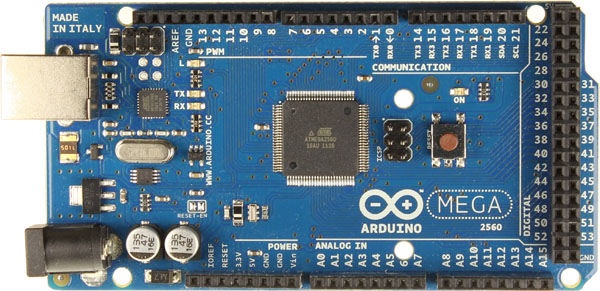
\includegraphics[width=5cm]{gambar/arduino_mega.jpg}
	\caption{Arduino Mega 2560}
\end{figure}

Arduino Mega 2560 memuat semua yang dibutuhkan untuk mendukung kerja dari sebuah mikrokontroler. Arduino Mega 2560 dapat dengan mudah dioperasikan untuk pengaplikasian ke sebuah sistem kerja karena dapat dihubungkan dengan kabel USB sebagai komunikasinya. Untuk powernya, Arduino Mega 2560 dapat dihidupkan melalui jack DC yang dipunyainya dengan diberi tegangan DC, dapat dengan adapter DC atau baterai dengan nilai tegangan sesuai dengan spesifikasi pada Arduino. Spesifikasi Arduino Mega 2560 ditunjukkan pada Tabel 2.4
\begin{table}[H]
	\centering
	\caption{ Spesifikasi Arduino Mega 2560 }
	\resizebox{12cm}{!}{%
		\begin{tabular}{|l|l|}
		\hline
		Mikrokontroler     & Atmega2560$$\hspace{2cm} 		\\ \hline
		Tegangan operasional     & 5 V$$  				\\ \hline
		Tegangan masukan  & 5-12 V$$  		\\ \hline
		Pin digital I/O       & 54 (15 pin untuk keluaran PWM) $$   \\\hline
		Pin analog masukan     & 16$$ 		\\ \hline
		Arus DC per Pin I/O  & 20 mA $$   				\\ \hline
		Arus DC untuk Pin 3.3 V & 50 mA $$  				\\ \hline
		Memori flash    & 256 KB $$ 		\\ \hline
		Kecepatan clock & 16 MHz $$   				\\ \hline
		Dimensi & 101.52 x 53.3 mm $$  				\\ \hline
		
		\end{tabular}%
}
\end{table}

\section{Driver Motor H}
Driver Motor berfungsi sebagai pengontrol dari setiap pergerakan dari motor DC. Pergerakan seperti kecepata, arah putar serta lamanya pergerakan motor DC dapat dikontrol oleh sebuah driver motor. Driver Motor memiliki beberapa jenis tergantung dari spesifikasi dari motor DC yang digunaan. Salah satu jenis driver motor adalah driver motor EMS 30A H-Bridge. Bentuk fisik dari driver motor EMS 30A H-Bride dapat ditunjukkan pada Gambar 2.3

	\begin{figure}[H]
	\centering
	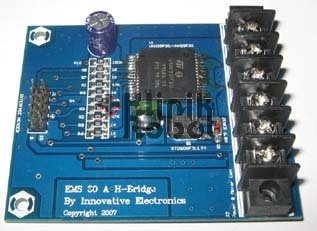
\includegraphics[width=5cm]{gambar/driver_motor.jpg}
	\caption{Driver Motor EMS 30A H-Bridge}
	\end{figure}

Driver Motor EMS 30A H-Bridge merupakan driver motor yang dapat mengoperasikan sebuah Motor DC dengan batasan arus hingga 30 Ampere. Driver ini memiliki 10 buah pin data yang dapat dihubungkan dengan sebuah mikrokontroler. Alokasi pin Driver Motor EMS 30A H-Bridge ini ditunjukkan pada tabel 2.12
% Please add the following required packages to your document preamble:
% \usepackage[normalem]{ulem}
% \useunder{\uline}{\ul}{}
\begin{table}[]
	\centering
	\caption{ Pin Driver Motor EMS 30A H-Bridge}
	\begin{tabular}{|c|c|c|l|}
		\hline
		Pin  & Nama & I/O & \multicolumn{1}{c|}{Fungsi}                                                                                                                                             \\ \hline
		1    & MIN1 & I   & Pin input untuk menentukan output MOUT1                                                                                                                                 \\ \hline
		2    & MIN2 & I   & Pin input untuk menentukan output MOUT2                                                                                                                                 \\ \hline
		3    & MEN1 & I/O & \begin{tabular}[c]{@{}l@{}}Pin enable untuk output MOUT1\\ Diberi logika High untuk mengkatifkan half H-Bridge 1, \\ diberi logika Low untuk menonaktifkan\end{tabular} \\ \hline
		4    & MEN2 & I/O & \begin{tabular}[c]{@{}l@{}}Pin enable untuk output MOUT2\\ Diberi logika High untuk mengkatifkan hal H-Bridge 2,\\ diberi logika Low untuk menonaktifkan\end{tabular}   \\ \hline
		5    & MSC  & O   & \begin{tabular}[c]{@{}l@{}}Output tegangan analog yang berbanding lurus dengan arus beban\\ (Range output 0-5 V) Tersedia untuk IC VNH2SP30\end{tabular}                \\ \hline
		6    & MPWM & I   & Pin input untuk mengatur kerja modul H-Bridge secara PWM                                                                                                                \\ \hline
		7,9  & VCC  & -   & Terhubung ke catu daya untuk input (5 Volt)                                                                                                                             \\ \hline
		8,10 & PGND & 0   & Titik referensi untuk caru daya input                                                                                                                                   \\ \hline
	\end{tabular}
\end{table}
\section{Processing Integrated Development Environment (IDE)}
Processing IDE adalah pemrograman sederhana yang diciptakan untuk pengembangan aplikasi yag berorientasi visual atau pencitraan dengan penekanan pada animasi dan memberi pengguna umpan balik melalui interaksi antarmuka. Para developer Processing IDE ini menginginkan sebuah cara untuk "membuat sketsa" gagasan dalam bentuk kode. Karena pemrograman telah berkembang selama beberapa dekade terakhir, Processing IDE telah mulai digunakan untuk pekerjaan tingkat produksi yang lebih maju. Awalnya dibangun sebagai ekstensi khusus domain Java yang ditargetkan untuk seniman dan desainer, Processing IDE telah berkembang menjadi alat desain dan prototipe lengkap dan penuh yang digunakan untuk pekerjaan instalasi skala besar, grafis gerak, dan visualisasi data yang rumit. Tampilan pada Processing IDE ditunjukkan pada gamba 3.1
	\begin{figure}[H]
	\centering
	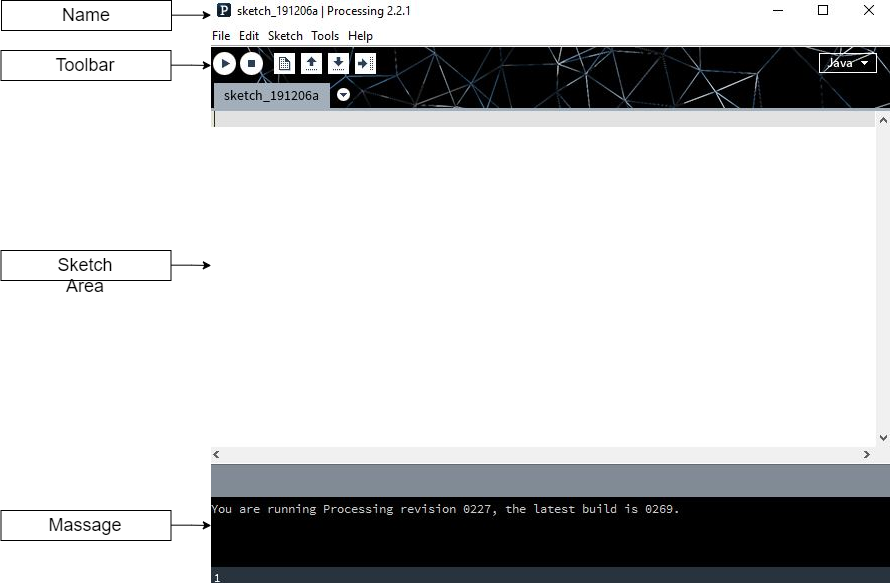
\includegraphics[width=10cm]{gambar/processing_view.png}
	\caption{Processing IDE}
\end{figure}


\subsection{Syntax dalam Processing IDE }

\subsubsection{Mengatur ukuran}
Ukuran sebuah objek pada processing IDE diatur menggunakan sebuah syntax size() Fungsi size() digunakan untuk menetapkan variabel global lebar dan tinggi dari suatu program. Ukuran untuk panjang dan tinggi tersebut menggunakan ukuran piksel. Lebar diwakili dengan variabel "width" dan tinggi diwakili dengan variabel. Untuk objek yang ukurannya tergantung pada layar, selalu gunakan variabel ebar dan tinggi, bukan angka. Ini mencegah masalah saat parameter fungsi size() diubah. Berikut penulisan dari fungsi size() untuk menetapkan lebar dan tinggi suatu program:  size(1000, 1000); 

\subsubsection{Shape}
Shape adalah syntax pada Processing IDE yang berfungsi untuk membuat berbagai macam bentuk, seperti persegi panjang, lingkaran, garis, dan bentuk lainnya yang dapat diatur ukurannya dengan parameter-parameter tertentu. Tabel 2.4 merupakan contoh dari beberapa syntax shape. 
\begin{table}[]
	\centering
	\caption{\emph Syntax Shape}
	\begin{tabular}{|l|l|l|l|}
		\hline
		
		No & Sytax                          & Bentuk & Keterangan                                                                                                                                                                                    \\ \hline
		1  & ellipse(a,b,c,d)               &        & \begin{tabular}[c]{@{}l@{}}a = koordinatX \\ b = koordinatY \\ c= lebar diameter \\ d= tinggi diameter\end{tabular}                                                                           \\ \hline
		2  & arc(a,b,c,d,start,st op,moode) &        & \begin{tabular}[c]{@{}l@{}}a = koordinatX \\ b = koordinatY \\ c = lebar diameter \\ d = tinggi diameter \\ start = sudut mulai \\ stop = sudut akhir \\ mode = PIE, CHORD, OPEN\end{tabular} \\ \hline
		3  & line(x1,y1,x2,y2)              &        & \begin{tabular}[c]{@{}l@{}}x1 = koordinatX1 \\ y1 = koordinatY1 \\ x2 = koordinatX2 \\ y2 = koordinatY2\end{tabular}                                                                          \\ \hline
		4  & point(x,y)                     &        & \begin{tabular}[c]{@{}l@{}}x = koordinatX \\ y = koordinatY\end{tabular}                                                                                                                      \\ \hline
		5  & rect(a,b,c,d,r)                &        & \begin{tabular}[c]{@{}l@{}}a = koordinatX1 \\ b = koordinatY1 \\ c = koordinatX2 \\ d= koordinatY1\end{tabular}                                                                               \\ \hline
	\end{tabular}
\end{table}
\subsubsection{Transformasi Bentuk Pada Processing IDE }
Transformasi pada Processing IDE digunakan untuk memindahkan, memutar atau, mengecilkan atau membesarkan suatu objek dan perpindahannya dapat diatur dengan parameter-parameter tertentu di dalam Processing IDE. Transformasi adalah dasar dari pemrograman Processing IDE. Tabel 2.5  adalah adalah contoh penulisan syntax dari Transformasi. 

\begin{table}[]
		\centering
	\caption{\emph Syntax Transformasi}
	\begin{tabular}{|c|l|l|}
		\hline
		No & \multicolumn{1}{c|}{\textit{Syntax}} & \multicolumn{1}{c|}{Keterangan}                                                            \\ \hline
		1  & Translate(x,y)                       & \begin{tabular}[c]{@{}l@{}}x = transisi kiri/kanan \\ y = transisi atas/bawah\end{tabular} \\ \hline
		2  & Rotate(angle)                        & angle=besar sudut rotasi(radian                                                            \\ \hline
		3  & RotateX(angle)                       & angle=besar sudut rotasi(radian)                                                           \\ \hline
		4  & RotateY(angle)                       & angle=besar sudut rotasi(radian)                                                           \\ \hline
		5  & Rotatez(angle)                       & angle=besar sudut rotasi(radian)                                                           \\ \hline
		6  & Scale(S)                             & s = besar pengecilan pembesaran (%)                                                        \\ \hline
	\end{tabular}
\end{table}
\subsubsection{Akses Koordinat Mouse }
Processing IDE mempunyai fungsi khusus yaitu dapat melacak posisi mouse baik secara vertical maupun horizontal. Akan tetapi Processing IDE hanya dapat melacak posisi mouse saat sketch dijalankan saja. Nilai default mouseX dan mouseY adalah 0, jadi 0 akan dikembalikan sampai mouse bergerak di depan jendela sketsa. (ini biasanya terjadi saat sketsa dijalankan pertama kali). Setelah mouse bergerak menjauh dari jendela, mouseX akan terus melaporkan posisi terakhirnya. Tabel 2.6  adalah contoh penulisan syntax dari mouse. 
\begin{table}[]
		\centering
	\caption{\emph Syntax Koordinat Mouse}
	\begin{tabular}{|c|l|l|}
		\hline
		No & \multicolumn{1}{c|}{\textit{Syntax}} & \multicolumn{1}{c|}{Keterangan}                                                                                                 \\ \hline
		1  & mouseX                               & \begin{tabular}[c]{@{}l@{}}Variabel sistem X memiliki nilai dari \\ koordinat horizontal mouse secara real time\end{tabular}    \\ \hline
		2  & mouseY                               & \begin{tabular}[c]{@{}l@{}}Variabel sistem Y memiliki nilai dari koordinat \\ horizontal mouse secara real time.\end{tabular}   \\ \hline
		3  & mouseButton()                        & \begin{tabular}[c]{@{}l@{}}Bila tombol mouse ditekan, nilai variable sistem \\ disetel ke LEFT,RIGHT, atau CENTER.\end{tabular} \\ \hline
		4  & mouseClicked()                       & \begin{tabular}[c]{@{}l@{}}Dipanggil setelah tombol mouse ditekan \\ dan kemudian dilepaskan.\end{tabular}                      \\ \hline
		5  & mouseDragged()                       & Dipanggil setelah tombol mouse bergerak saat ditekan.                                                                           \\ \hline
	\end{tabular}
\end{table}

\subsubsection{ Compile Sketch }
rogram pada Processing IDE dinamakan sketch. Tujuan diberi nama sketch adalah untuk membuat pemrograman bergaya Java ini terasa lebih seperti scripting, dan mengadopsi proses scripting untuk menulis kode dengan cepat. Sketch disimpan dalam bentuk Sketchbook, folder yang digunakan sebagai default menyimpanan semua proyek Processing IDE. Sketch yang tersimpan dalam Sketchbook dapat diakses dari File - Sketchbook. Sebagai alternatif, File - Open.. dapat digunakan untuk membuka sketch dari tempat lain pada sistem. Gambar 2. 21 adalah opsi toolbar untuk menjalankan sketch. Run (Ctrl + R) adalah opsi untuk menjalankan sketch yang telah dibuat, begitu pula dengan Tweak. Present (Ctrl + Shift + R) berfungsi untuk menjalankan sketch dengan layer penuh (Fullscreen). Stop berfungsi untuk menghentikan sketch. 

	\begin{figure}[H]
	\centering
	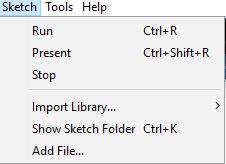
\includegraphics[width=5cm]{gambar/compile.jpg}
	\caption{Toolbar \emph Sketch}
\end{figure}

\subsection{\emph Library untuk Processing IDE }
\subsubsection{ Memuat Huruf (Font) pada Processing IDE }
Pfont adalah class yang digunakan untuk penggunaan font pada Processing IDE. Untuk membuat font yang akan digunakan dengan Processing IDE, dengan memilih "Create Font ..." dari menu Tools. Ini akan membuat font dalam format Processing IDE yang membutuhkan dan juga menambahkannya ke direktori data sketsa saat ini. Pengolahan menampilkan font menggunakan format font .vlw. Fungsi loadFont() digunakan untuk membuat font baru dan textFont () digunakan agar font baru yang telah dibuat tersebut aktif. Syntax list() berfungsi untuk membuat daftar font yang terinstal di komputer, yang merupakan informasi yang berguna untuk digunakan dengan fungsi createFont () untuk mengubah font secara dinamis menjadi format yang bisa digunakan di Processing IDE. 


\subsubsection{ Memuat ControlP5 pada Processing IDE }
ControlP5 adalah library yang berfungsi sebagai pengontrol untuk membuat antarmuka dengan user, ControlP5 berupa grafis di dalam sketch Processing IDE yang meliputi Slider, Button, Toggles, Knobs, Radiobutton, dan dapat dengan mudah ditambahkan ke sketch pengolahan. ControlP5 ditulis oleh Andreas Schlegel untuk pemrograman Processing IDE. Library ControlP5 bisa diunduh di laman https://github.com/sojamo/controlp5, atau unduh di library Processing IDE secara langsung. 

